
\bta{2021}


\section{Use of English}

\noindent
\textbf{Directions:}\\
Read the following text. Choose the best word (s) for each numbered
	blank and mark A, B, C or D on the ANSWER SHEET.
	(10 points)


\TiGanSpace



	Fluid intelligence is the type of intelligence that has to do with
	short-term memory and the ability to think quickly, logically, and
	abstractly in order to solve new problems. It \cloze in young
	adulthood, levels out for a period of time, and then \cloze starts to
	slowly decline as we age. But \cloze aging is inevitable, scientists
	are finding that certain changes in brain function may not be.
	
	One study found that muscle loss and the \cloze of body fat around the
	abdomen are associated with a decline in fluid intelligence. This
	suggests the \cloze that lifestyle factors might help prevent or
	\cloze this type of decline.
	
	The researchers looked at data that \cloze measurements of lean
	muscle and abdominal
	fat from more than 4, 000 middle-to-older-aged men and women and
	\cloze that data to reported changes in fluid intelligence over a
	six-year period. They found that middle-aged people
	\cloze higher measures of abdominal fat \cloze worse on
	measures of fluid intelligence as the years \cloze.
	
	For women, the association may be \cloze to changes in immunity
	that resulted from excess abdominal fat; in men, the immune system did
	not appear to be \cloze. It is hoped that future studies could
	\cloze these differences and perhaps lead to different
	\cloze for men and women.
	
	\cloze , there are steps you can \cloze to help reduce
	abdominal fat and maintain lean muscle mass as you age in order to
	protect both your physical and mental \cloze. The two highly
	recommended lifestyle approaches are maintaining or increasing your
	\cloze of aerobic exercise and following a Mediterranean-style
	\cloze that is high in fiber and eliminates highly processed
	foods.


\newpage

\begin{enumerate}
	%\renewcommand{\labelenumi}{\arabic{enumi}.}
	% A(\Alph) a(\alph) I(\Roman) i(\roman) 1(\arabic)
	%设定全局标号series=example	%引用全局变量resume=example
	%[topsep=-0.3em,parsep=-0.3em,itemsep=-0.3em,partopsep=-0.3em]
	%可使用leftmargin调整列表环境左边的空白长度 [leftmargin=0em]
	\item
\fourchoices
{pauses}
{returns}
{peaks}
{fades}

	

\item 			
\fourchoices
{alternatively}
{formally}
{accidentally}
{generally}


			
\item
			
\fourchoices
{while}
{since}
{once}
{until}

	
\item 
\fourchoices
{detection}
{accumulation}
{consumption}
{separation}


\item
			
\fourchoices
{possibility}
{decision}
{goal}
{requirement}

	
\item 
\fourchoices
{delay}
{ensure}
{seek}
{utilize}

	
\item 
\fourchoices
{modified}
{supported}
{included}
{predicted}

	
\item 
\fourchoices
{devoted}
{compared}
{converted}
{applied}

	
\item 
\fourchoices
{with}
{above}
{by}
{against}

	
\item 
\fourchoices
{lived}
{managed}
{scored}
{played}

	
\item 
\fourchoices
{ran out}
{set off}
{drew in}
{went by}

	
\item 
\fourchoices
{superior}
{attributable}
{parallel}
{resistant}

	
\item 
\fourchoices
{restored}
{isolated}
{involved}
{controlled}

	
\item 
\fourchoices
{alter}
{spread}
{remove}
{explain}

	
\item 
\fourchoices
{compensations}
{symptoms}
{demands}
{treatments}

	
\item 
\fourchoices
{Likewise}
{Meanwhile}
{Therefore}
{Instead}

	
\item 
\fourchoices
{change}
{watch}
{count}
{take}

	
\item 
\fourchoices
{well-being}
{process}
{formation}
{coordination}

	
\item 
\fourchoices
{level}
{love}
{knowledge}
{space}

\item 
\fourchoices
{design}
{routine}
{diet}
{prescription}


\end{enumerate}


\vfil

\section{Reading Comprehension}



\noindent
\textbf{Part A}\\
\textbf{Directions:}\\
Read the following four texts. Answer the questions after each
text by choosing A, B, C or
D. Mark your answers
on the ANSWER SHEET. (40 points)


\newpage
\subsection{Text 1}



How can the train operators possibly justify yet another increase to
rail passenger fares? It has become a grimly reliable annual ritual:
every January the cost of travelling by train rises, imposing a
significant extra burden on those who have no option but to use the rail
network to get to work or otherwise. This year's rise, an average of 2.7
percent, may be a fraction lower than last year's, but it is still well
above the official Consumer Price Index (CPI) measure of inflation.

Successive governments have permitted such increases on the grounds that
the cost of investing in and running the rail network should be borne by
those who use it, rather than the general taxpayer. Why, the argument
goes, should a car-driving pensioner from Lincolnshire have to subsidise
the daily commute of a stockbroker from Surrey? Equally, there is a
sense that the travails of commuters in the South East, many of whom
will face among the biggest rises, have received too much attention
compared to those who must endure the relatively poor infrastructure of
the Midlands and the North.

However, over the past 12 months, those commuters have also experienced
some of the worst rail strikes in years. It is all very well train
operators trumpeting the improvements they are making to the network,
but passengers should be able to expect a basic level of service for the
substantial sums they are now paying to travel. The responsibility for
the latest wave of strikes rests on the unions. However, there is a
strong case that those who have been worst affected by industrial action
should receive compensation for the disruption they have suffered.

The Government has pledged to change the law to introduce a minimum
service requirement so that, even when strikes occur, services can
continue to operate. This should form part of a wider package of
measures to address the long-running problems on Britain's railways.
Yes, more investment is needed, but passengers will not be willing to
pay more indefinitely if they must also endure cramped, unreliable
services, punctuated by regular chaos when timetables are changed, or
planned maintenance is managed incompetently. The threat of
nationalisation may have been seen off for now, but it will return with
a vengeance if the justified anger of passengers is not addressed in
short order.

\vspace{1em}

\begin{enumerate}[resume]
	%\renewcommand{\labelenumi}{\arabic{enumi}.}
	% A(\Alph) a(\alph) I(\Roman) i(\roman) 1(\arabic)
	%设定全局标号series=example	%引用全局变量resume=example
	%[topsep=-0.3em,parsep=-0.3em,itemsep=-0.3em,partopsep=-0.3em]
	%可使用leftmargin调整列表环境左边的空白长度 [leftmargin=0em]
	\item
The author holds that this year's increase in rail passengers fares \lineread.


\fourchoices
{will ease train operation's burden}
{has kept pace with inflation}
{is a big surprise to commuters}
{remains an unreasonable measure}


\item
The stockbroker in Para. 2 is used to stand for \lineread.


\fourchoices
{car drivers}
{rail travellers}
{local investors}
{ordinary tax payers}


\item
 It is indicated in Para. 3 that train operators \lineread.


\fourchoices
{are offering compensations to commuters}
{are trying to repair ralations with the unions}
{have failed to provide an adequate source}
{have suffered huge losses owing to the strikes}


\item
If unable to calm down passengers, the railways may have to face \lineread.


\fourchoices
{the loss of investment}
{the collapse of operations}
{a reduction of revenue}
{a change of ownership}



\item
 Which of the following would be the best title for the text?


\fourchoices
{Who Are to Blame for the Strikes?}
{Constant Complaining Doesn't Worlk}
{Can Nationalization Bring Hope?}
{Ever-rising Fares Aren't Sustainable	}

	
\end{enumerate}





\newpage
\subsection{Text 2}



Last year marked the third year in a row of when Indonesia's bleak rate
of deforestation has slowed in pace. One reason for the turnaround may
be the country's antipoverty program.

In 2007, Indonesia started phasing in a program that gives money to its
poorest residents under certain conditions, such as requiring people to
keep kids in school or get regular medical care. Called conditional cash
transfers or CCTs, these social assistance programs are designed to
reduce inequality and break the cycle of poverty. They're already used
in dozens of countries worldwide. In Indonesia, the program has provided
enough food and medicine to substantially reduce severe growth problems
among children.

But CCT programs don't generally consider effects on the environment. In
fact, poverty alleviation and environmental protection are often viewed
as conflicting goals, says Paul Ferraro, an economist at Johns Hopkins
University.

That's because economic growth can be correlated with environmental
degradation, while protecting the environment is sometimes correlated
with greater poverty. However, those correlations don't prove cause and
effect. The only previous study analyzing causality, based on an area in
Mexico that had instituted CCTs, supported the traditional view. There,
as people got more money, some of them may have more cleared land for
cattle to raise for meat, Ferraro says.

Such programs do not have to negatively affect the environment, though.
Ferraro wanted to see if Indonesia's poverty-alleviation program was
affecting deforestation. Indonesia has the third-largest area of
tropical forest in the world and one of the highest deforestation rates.

Ferraro analyzed satellite data showing annual forest loss from 2008 to
2012---including during Indonesia's phase-in of the antipoverty
program---in 7, 468 forested villages across 15 provinces . 
 ``we see that the program is
associated with a 30 percent reduction in deforestation,'' Ferraro says.

That's likely because the rural poor are using the money as makeshift
insurance policies against inclement weather, Ferraro says. Typically,
if rains are delayed, people may clear land to plant more rice to
supplement their harvests. With the CCTs, individuals instead can use
the money to supplement their harvests.

Whether this research translates elsewhere is anybody's guess. Ferraro
suggests
the results may transfer to other parts of Asia, due to
commonalities such as the
 the importance of growing rice and market access. And
regardless of transferability, the study shows that what's good for
people may also be good for 
 the environment. Even if this program didn't
reduce poverty, Ferraro says, ``the value of the avoided deforestation just for
carbon dioxide emissions alone is more than the program costs.''


\begin{enumerate}[resume]
	%\renewcommand{\labelenumi}{\arabic{enumi}.}
	% A(\Alph) a(\alph) I(\Roman) i(\roman) 1(\arabic)
	%设定全局标号series=example	%引用全局变量resume=example
	%[topsep=-0.3em,parsep=-0.3em,itemsep=-0.3em,partopsep=-0.3em]
	%可使用leftmargin调整列表环境左边的空白长度 [leftmargin=0em]
	\item
According to the first two paragraphs, CCT programs aim to \lineread.


\fourchoices
{facilitate health care reform}
{help poor families get better off}
{improve local education systems}
{lower deforestation rates}


\item
 The study based on an area in Mexico is cited to show that \lineread.


\fourchoices
{cattle rearing has been a major means of livelihood for the poor}
{CCT programs have helped preserve traditional lifestyles}
{antipoverty efforts require the participation of local farmers}
{economic growth tends to cause environmental degradation}



\item
 In his study about Indonesia, Ferraro intends to find out \lineread.


\fourchoices
{its acceptance level of CCTs}
{its annual rate of poverty alleviation}
{the relation of CCTs to its forest loss}
{the role of its forests in climate change}



\item
According to Ferraro, the CCT program in Indonesia is most valuable
in that \lineread.


\fourchoices
{it will benefit other Asian countries}
{it will reduce regional inequality}
{it can protect the environment}
{it can boost grain production}


\item
What is the text centered on?


\fourchoices
{The effects of a program.}
{The debates over a program.}
{The process of a study.}
{The transferability of a study.	}

	
\end{enumerate}




\newpage
\subsection{Text 3}



As a historian, who's always searching for the text or the image that
makes us re-evaluate the past. I've become preoccupied with looking for
photographs that show our Victorian ancestors smiling (what better way
to shatter the image of 19th-century prudery?). I've found quite a few,
and---since I started posting them on Twitter---they have been causing
quite a stir. People have been surprised to see evidence that Victorians
had fun and could, and did, laugh. They are noting that the Victorians
suddenly seem to become more human as the hundred-or-so years that
separate us fade away through our common experience of laughter.

Of course, I need to concede that my collection of ``Smiling
Victorians'' makes up only a tiny percentage of the vast catalogue of
photographic portraiture created between 1840 and 1900, the majority of
which show sitters posing miserably and stiffly in front of painted
backdrops, or staring absently into the middle distance. How do we
explain this trend?

During the 1840s and 1850s, in the early days of photography, exposure
times were notoriously long: the daguerreotype photographic method
(producing an image on a silvered copper plate) could take several
minutes to complete, resulting in blurred images as sitters shifted
position or adjusted their limbs. The thought of holding a fixed grin as
the camera performed its magical duties was too much to contemplate, and
so a non-committal blank stare became the norm.

But exposure times were much quicker by the 1880 s, and the introduction
of the Box Brownie and other portable cameras meant that, though slow by
today's digital standards, the exposure was almost instantaneous.
Spontaneous smiles were relatively easy to capture by the 1890 s, so we
must look elsewhere for an explanation of why Victorians still hesitated
to smile.

One explanation might be the loss of dignity displayed through a cheesy
grin. ``Nature gave us lips to conceal our teeth,'' ran one popular
Victorian maxim, alluding to the fact that before the birth of proper
dentistry, mouths were often in a shocking state of hygiene. A flashing
set of healthy and clean, regular ``pearly whites'' was a rare sight in
Victorian society, the preserve of the super-rich (and even then, dental
hygiene was not guaranteed).

A toothy grin (especially when there were gaps or blackened gnashers)
lacked class: drunks, tramps, prostitutes and buffoonish music hall
performers might gurn and grin with a smile as wide as Lewis Carroll's
gum-exposing Cheshire Cat, but it was not a becoming look for properly
bred persons. Even Mark Twain, a man who enjoyed a hearty laugh, said
that when it came to photographic portraits there could be ``nothing
more damning than a silly, foolish smile fixed forever''.


\begin{enumerate}[resume]
	%\renewcommand{\labelenumi}{\arabic{enumi}.}
	% A(\Alph) a(\alph) I(\Roman) i(\roman) 1(\arabic)
	%设定全局标号series=example	%引用全局变量resume=example
	%[topsep=-0.3em,parsep=-0.3em,itemsep=-0.3em,partopsep=-0.3em]
	%可使用leftmargin调整列表环境左边的空白长度 [leftmargin=0em]
	\item
According to Paragraph 1, the author's posts on Twitter \lineread.


\fourchoices
{illustrated the development of Victorian photography}
{highlighted social media's role in Victorian studies}
{re-evaluated the Victorian's notion of public image}
{changed people's impression of the Victorians}


\item
What does the author say about the Victorian portraits he has
collected?


\fourchoices
{They are rare among photographs of that age.}
{They show effects of different exposure times.}
{They mirror 19th-century social conventions.}
{They are in popular use among historians.}



\item
 What might have kept the Victorians from smiling for pictures in the
1890s?


\fourchoices
{Their inherent social sensitiveness.}
{Their tension before the camera.}
{Their distrust of new inventions.}
{Their unhealthy dental condition.}



\item
Mark Twain is quoted to show that the disapproval of smiles in
pictures was \lineread.


\fourchoices
{a deep-root belief}
{a misguided attitude}
{a controversial view}
{a thought-provoking idea}


\item
Which of the following questions does the text answer?


\fourchoices
{Why did most Victorians look stern in photographs?}
{Why did the Victorians start to view photographs?}
{What made photography develop slowly in the Victorian period?}
{How did smiling in photographs become a post-Victorian norm?	}
	
	
\end{enumerate}



\newpage
\subsection{Text 4}



From the early days of broadband, advocates for consumers and web-based
companies worried that the cable and phone companies selling broadband
connections had the power and incentive to favor their own or their
partners' websites and services over those of their rivals. That's why
there has been such a strong demand for rules that would prevent
broadband providers from picking winners and losers online, preserving
the freedom and innovation that have been the lifeblood of the internet.

Yet that demand has been almost impossible to fill---in part because
of pushback from broadband providers, anti-regulatory conservatives and
the courts. A federal appeals court weighed in again Tuesday, but
instead of providing a badly needed resolution, it only prolonged the
fight. At issue before the U.S. Court of Appeals for the District of
Columbia Circuit was the latest take of the Federal Communications
Commission (FCC) on net neutrality, adopted on a party-line vote in 2017. The
Republican penned order not only eliminated the strict net neutrality
rules the FCC had adopted when it had a Democratic majority in 2015, but
rejected the commission's authority to require broadband providers to do
much of anything. The order also declared that state and local
governments couldn't regulate broadband providers either.

The commission argued that other agencies would protect against
anti-competitive behavior, such as a broadband-providing conglomerate
like AT\&T favoring its own video-streaming service at the expense of
Netflix and Apple TV. Yet the FCC also ended the investigations of
broadband providers that imposed data caps on their rivals' streaming
services but not their own.

On Tuesday, the appeals court unanimously upheld the 2017 order
deregulating broadband providers, citing a Supreme Court ruling from
2005 that upheld a similarly deregulatory move. But Judge Patricia
Millett rightly argued in a concurring opinion that ``the result is
unhinged from the realities of modern broadband service,'' and said
Congress or the Supreme Court could intervene to ``avoid trapping
Internet regulation in technological anachronism.''

In the meantime, the court threw out the FCC's attempt to block all
state rules on net neutrality, while preserving the commission's power
to pre-empt individual state laws that undermine its order. That means
more battles like the one now going on between the Justice Department
and California, which enacted a tough net neutrality law in the wake of
the FCC's abdication.

The endless legal battles and back-and-forth at the FCC cry out for
Congress to act. It needs to give the commission explicit authority once
and for all to bar broadband providers from meddling in the traffic on
their network and to create clear rules protecting openness and
innovation online.

\begin{enumerate}[resume]
	%\renewcommand{\labelenumi}{\arabic{enumi}.}
	% A(\Alph) a(\alph) I(\Roman) i(\roman) 1(\arabic)
	%设定全局标号series=example	%引用全局变量resume=example
	%[topsep=-0.3em,parsep=-0.3em,itemsep=-0.3em,partopsep=-0.3em]
	%可使用leftmargin调整列表环境左边的空白长度 [leftmargin=0em]
	\item
There has long been concern that broadband provides would \lineread.


\fourchoices
{bring web-based firms under control}
{slow down the traffic on their network}
{show partiality in treating clients}
{intensify competition with their rivals}


\item
Faced with the demand for net neutrality rules, the FCC \lineread.


\fourchoices
{sticks to an out-of-date order}
{takes an anti-regulatory stance}
{has issued a special resolution}
{has allowed the states to intervene}



\item
What can be learned about AT\&T from Paragraph 3?


\fourchoices
{It protects against unfair competition}
{It engages in anti-competitive practices.}
{It is under the FCC'S investigation.}
{It is in pursuit of quality service.}


\item
Judge Patricia Millett argues that the appeals court's decision \lineread.


\fourchoices
{focuses on trivialities}
{conveys an ambiguous message}
{is at odds with its earlier rulings}
{is out of touch with reality}


\item
What does the author argue in the last paragraph?


\fourchoices
{Congress needs to take action to ensure net neutrality.}
{The FCC should be put under strict supervision.}
{Rules need to be set to diversify online services.}
{Broadband providers' rights should be protected.}
	
	
	
\end{enumerate}



\newpage

\noindent
\textbf{Part B}\\
\textbf{Directions:}\\
In the following text, some sentences have been removed. For
questions 41--45, choose the most suitable one from the list A--G to fit
into each of numbered blanks. There are two extra choices, which do not
fit in any of the blanks. Mark your answers on the ANSWER SHEET. (10
points)


\TiGanSpace

In the movies and on television, artificial intelligence (AI) is
typically depicted as something sinister that will upend our way of
life. When it comes to AI in business, we often hear about it in
relation to automation and the impending loss of jobs, but in what ways
is AI changing companies and the larger economy that don't involve
doom-and-gloom mass unemployment predictions?

A recent survey of manufacturing and service industries from Tata
Consultancy Services found that companies currently use AI more often in
computer-to-computer activities than in automating human activities. 
Here are a few other ways AI is aiding companies without replacing
employees:



\textbf{Better hiring practices}


Companies are using artificial intelligence to remove some of the
unconscious bias from hiring decisions. ``There are experiments that
show that, naturally, the results of interviews are
much more biased than what AI does,'' 
says Pedro Domingos, author of \emph{The Master Algorithm: How the
	Qust for the Ultimate Learning Machine Will Remake Our World} and a
computer science professor at the University of Washington. In addition,
``  \linefill. '' One company that's doing this
is called Blendoor. It uses analytics to help identify where there may be bias
in the hiring process.



\textbf{More effective marketing}


Some AI software can analyze and optimize marketing email subject lines
to increase open rates. One company in the UK, Phrasee, claims their
software can outperform humans by up to 10 percent when it comes to
email open rates. This can mean millions more in revenue. 
\linefill.
These are ``tools that help people use data, not a replacement for
people,'' says Patrick
H. Winston, a professor of artificial
intelligence and computer science at MIT.



\textbf{Saving customers money}


Energy companies can use AI to help customers reduce their electricity
bills, saving them money while helping the environment. Companies can
also optimize their own energy use and cut down on the cost of
electricity. Insurance companies, meanwhile, can base their premiums on
AI models that more accurately access risk. Domingos says,  `` \linefill. ''




\textbf{Improved accuracy}


``Machine learning often provides a more reliable form of statistics,
which makes data more valuable,'' says Winston. It ``helps people make
smarter decisions.'' \\
\linefill.


\textbf{Protecting and Maintaining  infrastructure}


A number of companies, particularly in energy and transportation, use AI
image processing technology to inspect infrastructure and prevent
equipment failure or leaks before they happen. ``If they fail first and
then you fix them, it's very expensive,'' says Domingos. `` \linefill. ''



\begin{listmatch}
	%\renewcommand{\labelenumi}{\arabic{enumi}.}
	% A(\Alph) a(\alph) I(\Roman) i(\roman) 1(\arabic)
	%设定全局标号series=example	%引用全局变量resume=example
	%[topsep=-0.3em,parsep=-0.3em,itemsep=-0.3em,partopsep=-0.3em]
	%可使用leftmargin调整列表环境左边的空白长度 [leftmargin=0em]
	\item
I replace the boring parts of your job. If you're doing research, you
can have AI go out and look for relevant sources and information that
otherwise you just wouldn't have time for.

\item
There are also companies like Acquisio, which analyzes advertising
performance across multiple channels like Adwords, Bing and social
media and makes adjustments or suggestions about where advertising
funds will yield best results.


\item
One accounting firm, EY, uses an AI system that helps review contracts
during an audit. This process, along with employees reviewing the
contracts, is faster and more accurate.



\item
You want to predict if something needs attention now and point to
where it's useful for employees to go to.

\item
We're also giving our customers better channels versus picking up the
phone  to accomplish something beyond human scale.

\item
Before, they might not insure the ones who felt like a high risk or
charge them too much, or they would charge them too little and then it
would cost the company money.



\item
AI looks at résumés in greater numbers than humans would be able to,
and selects the more promising candidates.

\end{listmatch}


\newpage
\noindent
\textbf{Part C}\\
\textbf{Directions:}\\
Read the following text carefully and then translate the
underlined segments into Chinese. 
Write your answers on the ANSWER SHEET. (10 points)

\TiGanSpace

World War II was the watershed event for higher education in modern
western societies. \transnum \uline{Those societies came out of the war
with levels of enrollment that had been roughly constant at 3-5\% of the relevant age groups during the decades before
the war}. But after the war, great social and political changes arising
out of the successful war against Fascism created a growing demand in
European and American economies for increasing numbers of graduates with
more than a
secondary school education. \transnum \uline{And the demand that rose in
those societies for entry to higher education extended to groups and social classes that had not
thought of attending to a university before the war}. These demands resulted in a very rapid
expansion of the systems of higher education, beginning in the 1960s and
developing very rapidly (though unevenly) during the 1970s and 1980s.



The growth of higher education manifests itself in at least three quite
different ways, and these in turn have given rise to different sets of
problems. There was first  \emph{the rate of growth}: \transnum \uline{in many
countries of Western Europe the numbers of students in higher education
doubled within five-year periods during the decade of the 1960s and doubled
again in seven, eight, or 10 years by the middle of the 1970 s}. Second, growth obviously affected
the \emph{absolute size} both of systems and individual institutions.
And third, growth was reflected in changes in \emph{the proportion of
the relevant age group} enrolled in institutions of higher education.

Each of these manifestations of growth carried its own peculiar
problems in its wake. For example, a high growth rate placed great strains
on the existing structures of governance, of administration, and above all of
socialization. When a faculty or department grows from, say, five to 20
members within three or four years, \transnum \uline{and when the new staff are
predominantly young men and women fresh from postgraduate study, they
largely define the norms of academic life in that faculty.} And if the
postgraduate student population also grows rapidly and there is loss of a
close apprenticeship relationship between faculty members and students,
the student culture becomes the chief socializing force for new postgraduate
students, with consequences for the intellectual and academic life of the
institution---this was seen in America as well as in France, Italy, West
Germany, and Japan. \transnum  \uline{High growth rates increased the chances for
academic innovation; they also weakened the forms and processes by which
teachers and students are admitted into a community of scholars during
periods of stability or slow growth.} In the 1960s and 1970s, European
universities saw marked changes in their governance arrangements, with the
empowerment of junior faculty and to some degree of students as well.



\newpage

\section{Writing}



\noindent
\textbf{Part A}\\
\textbf{51. Directions:}


A foreign friend of yours has recently graduated from college and
intends to find a job in China. Write him/her an email to make some
suggestions.


You should write about 100 words on the ANSWER SHEET.



\textbf{Do not} use your own name in the email. Use `` Li Ming''
instead. (10 points)

\vspace{2em}

\noindent
\textbf{Part B}\\
\textbf{52. Directions:}



Write an essay of 160-200 words based on the pictures below. In
your essay, you should


\begin{listwrite}
	\item 
	describe the picture briefly,
	
	\item 
	interpret its intended meaning, and
	
	\item 
	give your comments.
\end{listwrite}

You should write neatly on the ANSWER SHEET. (20 points)


\begin{figure}[h!]
	\centering
	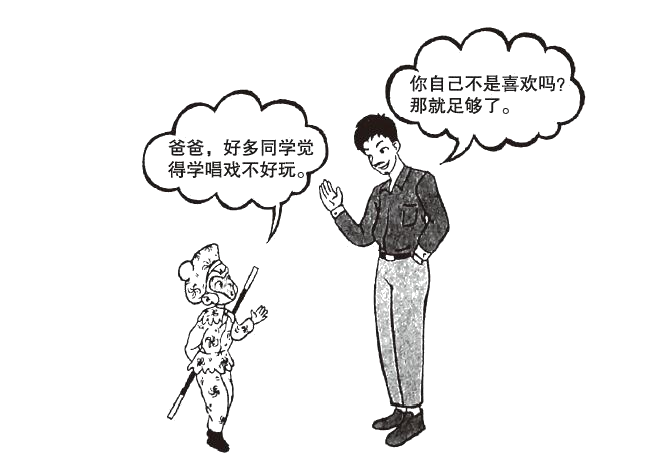
\includegraphics[width=0.64\linewidth]{picture/2021.png}
\end{figure}




